
\begin{savequote}[8cm]

    We hear a lot these days about genes and molecules, but how does one human brain, or one human being coordinate, or entrain, or resonate with another?  We may not realise it but we live in a world of coordination, at every level and every scale of endeavour.

  \qauthor{--- J. A. S. Kelso  \textit{Coordination and the Complimentary Nature} Presentation to the The New York Academy of Sciences - May 12, 2010}
\end{savequote}


%I do not see any way to avoid the problem of coordination and still understand the physical basis of life.
%\qauthor{--- H. H. Pattee  \textit{The role of instabilities in the evolution of control hierarchies} 1976}


\chapter{\label{chap:theory}Click and connection through joint action}

\minitoc

While it is now well-established that successful interpersonal entrainment of movement can be responsible for generate positive psychological and social effects, the mechanisms through which entrainment is achieved remain poorly understood.  As a response to the theoretical and empirical gaps in cognitive and evolutionary accounts of group exercise outlined in Chapter~\ref{chap:intro}, in this chapter I review strands of research capable of accounting for team click and social connection through joint action.  This review sets the foundation for a novel theory of social bonding through joint action, presented in the next chapter (Chapter~\ref{chap:theoryGE}).

In particular, I identify team click as a special case phenomenon of joint action and a potential mediator of the relationship between joint action and social bonding in group exercise contexts.  Emerging research from the social cognition of joint action suggests that a continuum of cognitive mechanisms are responsible for establishing and maintaining behavioural coordination between two or more individuals.

More efficient solutions to the cognitive uncertainty of joint action appear to involve reducing the cognitive demands associated with interoceptive predictive modelling and instead increasing reliance on more direct extra-neural coupling with the environment.  These mechanisms also appear to be modulated by inter-individual and cultural variation in knowledge, expertise, experience, and personality type.  Evidence suggests coordination in joint action can set the foundation for social connection, and the phenomenon of team click can be understood as an optimal state of interpersonal coordination in joint action that maximally activates a causal pathway between joint action and social bonding.  I conclude the chapter by summarising a theory of social bonding through joint action, and outlining predictions that arise from this theory.

%In this dissertation I attend specifically to the relationship between joint action and social bonding in the group exercise context of professional rugby in China.  In this chapter I formulate a novel theory of social bonding through joint action in order to address the knowledge gaps in the social high theory of group exercise and social bonding.


                                  \begin{CJK}{UTF8}{gbsn}

\section{The development of visceral agency in rugby's newest recruit\label{sect:SHW}}
Sun Hongwei arrived, escorted by his high school athletics coach, to the Beijing Temple of God of Agriculture Institute of Sport (hereafter the Institute) soon after I began my fieldwork in August 2015.  An 18-year-old with a slight build and timid demeanour---his gaze remained diverted to the ground during his first few months at the Institute---Hongwei later told me that he had never seen a rugby ball before that day he arrived.

Hongwei was from Hebei province, immediately surrounding the special prefecture of Beijing, China's capital.  Hongwei's coach had organised a trial for Hongwei with the Beijing Provincial men’s and women's Rugby Program (hereafter the Program) by calling upon social connections to the leadership of the Institute.  Athletes come to the Rugby Program from all over the country.  As I explain in more detail in Chapter~\ref{chap:researchSetting}, representing Beijing at a provincial level in a sport like rugby can translate into the opportunity to gain entrance to one of China's top universities and enhanced career employment opportunities thereafter.

Rugby is not a popular sport in China, but its recent inclusion in the Olympic games (in the form of the modified seven-a-side version of ``rugby sevens'') means that it now occupies a prominent place in the Chinese sport system.  Rugby programs such as the one at the Institute now exist in 12 of China's 34 provincial level regions, either embedded within, or somehow associated with, tertiary education institutions.  Thus, although rugby and China are not commonly associated terms, rugby now affords Chinese athletes a rare and under-capitalised opportunity to pursue attractive life-course opportunities of education and employment in an intensely competitive education system.

Without exception, the athletes who arrive at the Institute to join the rugby team were not like me; they had not spent their childhoods playing rugby in their schoolyards or watching professional rugby on television. Many who come to rugby transition from other more popular sports such as athletics, basketball, or association football, and often---like Hongwei---have never seen a rugby ball before they arrive.  Most athletes ``start from scratch,'' so to speak, in terms of their grasp of the requirements of the highly interactive and technically complex team sport.  In addition to complex patterns of movement coordination, rugby also involves unrestrained body-on-body collisions and intense bouts of high physiological exertion, requiring speed, strength, agility, and endurance to perform all of rugby's technical requirements successfully (see Chapter~\ref{chap:researchSetting} Section ~\ref{sect:rugbyUnion}).  Learning the game of rugby from a baseline of essentially zero, while also navigating the inevitably demanding social and political dynamics within the team and the Institute, was clearly going to be a daunting task for Hongwei.


                        \begin{center}
                          * * *
                        \end{center}

Hongwei was the first of the Program’s new recruits that I followed closely.  Even compared to other newly arrived junior athletes, he was noticeably timid and shy, particularly in his interactions with the coaches (myself included) and senior players. Nevertheless, Hongwei clearly signalled diligence and commitment through his participation in team activities.  He arrived early to each training session, and carried more than his fair share of the training equipment---a task shared by the most junior members of the team.  Each time I passed Hongwei in the corridors of the Institute he would greet me with a polite bow and greeting, ``Hello Coach'' (\textit{'jiaolian hao'} `教练好').  In these instances, Hongwei would coordinate his greeting with a moment's eye contact, only to return his gaze to the floor and continue walking.

Due to his lack of familiarity with the basic techniques of rugby, Hongwei was initially unable to fully participate in normal training with the rest of the team.  Instead, during the first month or so, Hongwei stood on the sidelines and practiced the basics with other athletes who were unable to fully participate in training due to injury.  He learning how to pass and catch the rugby ball, while stationary and running in-motion.  In my eyes at least---eyes of an observer accustomed to instinctual grasp of these movements from a young age---Hongwei's attempts to accustom himself with the skills of rugby were jarring.  The idiosyncrasies of rugby's ovular ball often foiled him.  I would regularly see him chasing after a ball on the ground he'd just fumbled, as if he was chasing in vein after a scurrying rabbit tactfully evading its pursuer.

                        \begin{center}
                          * * *
                        \end{center}

I interviewed Hongwei approximately six weeks after he arrived at the Institute.  Hongwei's demeanour during the interview was consistent with the timid and shy one that he presented publicly at training.  As explain below, he did show some signs of captivation with his new sport and social environment.  When I asked about his initial impressions of the on-field demands of rugby, however, Hongwei was quick to confess that he felt utterly unacquainted:

  \begin{quote}
    SHW: I still haven’t really started to practice any of the team plays or anything; all I can do so far is pass and run a little bit...(but) it's quite fun! \\
    JT: What do you think is the most difficult component of rugby? \\
    SHW: Um\textellipsis well, coordinating with teammates [on the field], particularly coordination in attack.  Because I can't figure it out.  When I first arrived, I didn’t even know what a ``switch play'' or a ``blocker play'' was.
  \end{quote}

  \begin{quote}
    SHW: 战术没怎么接触,就是像传球啊、跑动什么的会一点了 \\
    JT: 感觉怎么样?\\
    SHW: 挺好玩的!\\
    JT: 你认为橄榄球最难的一部分是什么? \\
    SHW: ...打配合,进攻的配合,因为搞不明白,刚来的时候也不知道什么交叉,后插什么的 \\
  \end{quote}

Hongwei was self-critical in this confession regarding his minimal grasp of the technical requirements of joint action in rugby.  The obvious stress and anxiety he expressed was indicative of a broader trend with the other athletes I interviewed, as I will explain in more detail in the ethnographic sections of this dissertation (see Chapters ~\ref{chap:ethnoField} \nobreakdash~\ref{chap:ethnoResults}). When athletes were asked in interviews about the most difficult aspect of rugby, on-field coordination with teammates was by far the most common answer, particularly among the new recruits and most junior athletes.

As I directed the interview towards topics beyond the on-field technical demands of rugby, Hongwei was more positive, framing rugby as an exciting new opportunity, and commenting that his friends and family were in awe of the fact that he is playing such an impressively ``strong'' physical sport like rugby.  When I asked him about something new that he had learnt through playing rugby, Hongwei automatically responded by emphasising the social dimensions to his experience at the Institute:

  \begin{quote}
    ...I think it's mainly this thing of having teammates. Before, when I was training for an individual sport, it was just me training by myself. [In that environment] it was a case of whoever trained well was successful.  But now with this team of brothers, elder teammates will take care of younger teammates. We all train together, and if you can’t do something, you can always ask your elder teammates...[Rugby] is so much better, because in an individual sport, if you can't master something, you have to go to your coach for help. Other athletes don't want to teach you, because if you surpass them, then they have to work even harder to keep up... I have had to learn about helping others, because rugby is not like an individual sport, where you look after your own performance and that's it.  In a team sport, if you don't do well, there's no need to get too frustrated or upset, because other athletes will help you out, and I will also help others out, that type of collaboration with each other.
  \end{quote}

\begin{CJK}{UTF8}{gbsn}
  \begin{quote}
    我觉得主要是师哥师弟的这一块儿,原来练个体项目都是自己练自己的,谁练好了谁厉害,但是现在师哥师弟,有师哥照顾师弟带着,互相练,我不会我可以问师哥
    ...因为个人项目你不会就必须要找教练,但是别人不愿意教你,因为你把别人超越了那别人还还得努力。 学到互相帮助,因为向个体项目自己成绩自己来拿就行,而像团体项目,即使自己做不好,也不用太泄气太沮丧,因为别人会帮你做好,我也会帮别人做好,互相协作的那种.
  \end{quote}
\end{CJK}

Hongwei's explicit reference to the collegiality of the team, and his position as junior member, highlights that the technical skills of rugby were not the only novel components of his experience.  Hongwei's background was in track and field (his event was pentathlon, very much an individual sport), and the team environment was completely new to him.  This was also the case for many of the other athletes in the team.  As I listened to his experiences associating rugby and group membership, I could not help but associate the quality of these explicit declarations of group membership with his overly mechanical imitation of rugby's foundational techniques.  In both I saw his willingness and desire to signal commitment; but both lacked---in the outset at least---a certain level of grasp or conviction.  In the case of his explicit celebration of rugby's social resources in interview, for example, I got the impression that Hongwei was telling me what he ought to believe or say, without actually deeply embodying or believing these things to be unequivocally true.


                            \begin{center}
                              * * *
                            \end{center}

A few months passed, and Hongwei continued to train.  He was as eager and committed as when he began, and I did notice some gradual improvement in his grasp of rugby's basic skills.  But he also remained extremely reserved, keeping his head low at all times in team settings, unless addressed by senior players or coaches.

Then, one evening when I had returned to my room in the Institute dormitory from a three week hiatus in Australia for Christmas, I heard a knock on my open door, and to my surprise Hongwei took an assertive stride into my room, carrying in two arms a draw-string bag containing rugby balls (which were in need of more air before the next day's training session).  Hongwei had never ventured into my room before, apart from when I invited him in for our first interview two months earlier---but certainly never before had he entered on his own accord.  Hongwei looked me straight in the eyes with his head held high and energy radiating from his face and upright chest.  I could not help but smile and ask, with genuine intrigue, ``How have you found training recently?''
``Very good'' he said, assertively and excitedly.  ``Much better than before.  At least now I know what’s going on at training, I can keep up with the plays!''  A big smile automatically grew on his face as he continued to hold my gaze confidently.  ``Oh good!'' I said, a little bit shocked.  I congratulated him for his hard work in training while I had been away, and encouraged him to keep at it.  At this, Hongwei took leave by bowing politely and saying ``Thanks coach.''  Wow, I remember thinking to myself, what quantity had all of a sudden possessed Hongwei? Was it possible that his diligent adherence to rugby over those first four months at the Institute had eventually instilled him with a visceral sense of agency?

                          \begin{center}
                            * * *
                          \end{center}


  %  the fact that aspects of Hongwei's personal and social demeanour at the Institute appeared to covary with his familiarity with the technical requirements of rugby over time suggests a relationship between joint action and group membership that is worthy of further investigation.
    %In the same way that Adrian's opening monologue (Chapter~\ref{chap:intro} Section ~\ref{sect:adrian}) suggested a relationship between the on-field dimensions of rugby and social processes between teammates, Hongwei's gradual development



\section{The need for a theory of joint action and social bonding in group exercise}

%HW's change is a change in attitude (Bateson) agency
How is it possible to scientifically account for the unmistakably visceral quality of Hongwei's transformation from timid newcomer to budding Beijing rugby player?  As the story of Hongwei anecdotally suggests, the visceral dimension of group exercise may take time to develop.  Presumably in Adrian (Chapter~\ref{chap:intro} Section ~\ref{sect:adrian}) I witnessed the finished product: through many years of on- and off-field engagement with the sport of rugby, Adrian came to embody rugby and thus profess its carnal mystery from a place of deep, intuitive knowing.  When I met him during my first stint of research at the Institute, Hongwei was only just beginning this journey.  But it became clear to me over an extended period of ethnographic research that with an increase in familiarity with the sport and the social details of the Institute came an increase in confidence, agency, and grasp.   As explained in the previous chapter, a scientific theory capable of accounting for the dynamic and interlocking physical, cognitive and social dimensions of the visceral mystery of group exercise is yet to be fully formulated.

In this chapter, I draw attention to strands of research capable of accounting for team click and social connection in joint action.  The theory proposed herein builds upon the hypothesis that group exercise is causally relevant to processes of social cohesion \citep{Dunbar2010,Whitehouse2014,Cohen2017}. In addition to ``cognitive'' processes (as they are narrowly defined by traditional ``stimulus-reponse'' paradigm \citep[e.g.][]{Marr1985}), recent empirical research programs within cognitive and evolutionary anthropology have begun to draw attention the role of physiological and affective mechanisms of neurobiological reward and autonomic arousal in shaping human behaviour, sociality, and cultural evolution.  As Dunbar and Shultz suggest, it is impossible to accept that humans merely adhere to a ``dung fly'' model of social aggregation; clear scientific evidence now suggests, rather, that humans have evolved a species-unique tendency to actively congregate and cohere around shared cultural practices \citep[cf.][]{Tomasello2005}.

But, as explained in Chapter~\ref{chap:intro}, existing approaches to the empirical question of human bondedness and social cohesion could benefit from a theoretical model of cognition in which physicality, emotion, information, and culture are more conceptually and causally integrated.  Doing so could help address empirical as well as theoretical gaps in our understanding of human sociality.  For example,  the social high theory of group exercise and social bonding \citep[cf.][]{Cohen2017} lacks a nuanced account of how extreme physiological cost generates profound meaning, or how cognitive complexity in joint action (beyond strict behavioural synchrony) can produce autotelic experiences of flow and team click (and flow on social effects, see Chapter~\ref{chap:intro} Section ~\ref{sect:empKnowGaps} for a more thorough explanation).  Likewise, in the case of the modes theory of ritual practice and social cohesion, an integrative model of cognition could facilitate empirical verification of a more continuous gradient of causal links between collective practices and social cohesion (see Chapter~\ref{chap:intro} Section ~\ref{sect:cogEvAnth} for a full elaboration).  In addition, despite best efforts to theorise the causal role of a fuller spectrum of ``factors of attraction,'' current models of cultural evolution (e.g., CAT, see Chapter~\ref{chap:intro} Section ~\ref{sect:cogEvAnth}) that underpin investigations of social cohesion remain entrenched in a theoretical debate that predominantly revolves around densely semantic cultural variants, i.e., ``representations.''  As such, more explicit cognitive mechanisms that facilitate social learning (e.g. imitation and instruction) are promoted in causal accounts of cultural evolution, while the implicit, embodied, and dynamical mechanisms of cultural transmission remain a subsidiary program of empirical research \citep{Lerique2016}.

Thus, in all three of these examples, proximate physical, cognitive, and social processes---while no doubt understood by researchers to be collectively relevant to human behavioural phenomena---are nonetheless treated theoretically as parallel and functionally distinct components.  A model of cognition that causally and systematically integrates cognitive processes with physiological and emotional processes could enable novel and testable predictions for a fuller spectrum of collective practices in human sociality.  In this dissertation, I propose that that an integrative model of cognition---``active inference'' \citep{Friston2010}---can assist empirical progress in the scientific of group exercise in human sociality, and indeed scientific questions relating to behaviour and evolution more broadly.

More so than most cultural variants that have traditionally formed the focus of scientific analysis, activities in which group exercise feature demand a dynamic conception of cognition.  Group exercise invariably involves brains and bodies engaged in ``in-the-moment'' and ``on-line'' joint action.  From a pure computational perspective, achieving and sustaining joint action is a daunting cognitive task, as it requires the coupling and constraining of various degrees of freedom belonging to autonomous co-actors \citep{Bernstein1967,Turvey1978}.  However, it is now more clearly understood that human cognition—--and indeed, cognition of biological life more generally—--does not rely on passive, ``brute force'' computation---like that of a digital computer---to manage to the challenges of interacting with the environment \citep{Yufik2013}.  Rather, prevailing theories of cognition suggest that humans flexibly deploy a range of ``active'' strategies in order to anticipate and regulate the uncertainty inherent in joint action and the universe of sensory causes more broadly \citep{Clark2015}.

In fact, one of the core cognitive strategies that has been overlooked by traditional ``stimulus-response'' models of cognition (which were inspired originally by digital computers) is physical movement itself.  The integration of movement into human inference through the ``Active Inference Framework'' \citep[hereafter AIF cf.][]{Friston2010} promises a clearer theoretical conception within which to conduct empirical research of the visceral, carnal, and embodied phenomena for which we have hitherto tended to collectively shroud in mystery, myth, and metaphysics \citep{Atran2010}, or else relegate to superordinate, supervening, or subsystemic causal status   \citep{Clark2015,Linson2018}.  Specifically, and for the purposes of this dissertation, AIF contains predictions for how humans click, connect, and cohere through joint action typical of group exercise contexts.

In this chapter, I use the AIF to develop testable predictions for a relationship between joint action and social bonding in group exercise.  In particular, I theorise team click as a psychological construct that mediates a relationship between joint action and social bonding.  While the social relevance of team click and the related concept of flow have evaded rigorous analysis within more traditional paradigms of social cognition \cite[for explanations as to why, see][]{Dietrich2004,Slingerland2014}, within the AIF, team click can be scientifically theorised as a special case in which the bonding effects of joint action are maximised.

%Preview theory here: As I outline in full detail in the sections below, a theory of social bonding through joint action depicts two or more brains

In the sections that follow in this chapter, I first introduce the cognitive challenge of joint action, and the suitability of team  click as a real-world empirical anchor and mediator of a relationship between joint action and social bonding (Section ~\ref{sect:dfProblem}).  I then introduce the AIF, including its three core tenets of thermodynamic cognition, predictive coding, and affordances (Sections ~\ref{sect:}\nobreakdash~\ref{sect:}).  With this grounding, I review attempts to apply AIF to joint action, and suggest that mechanisms of surprise (expectation violation), blurring of self and other agency, affective reward, and shared attention could give rise to experiences of team click and ground more elaborate processes of social identity and meaning making  (Section ~\ref{sect:}).  This review sets the foundation for the following chapter, in which I outline a novel theory of social bonding through joint action and suggest its suitability for explaining the relationship between group exercise and social cohesion.




\section{Human solutions to the challenge of joint action\label{sect:dfProblem}}
%\subsection{The degrees of freedom problem and its solutions in human movement}
Humans are hyper-social \citep{Tomasello2012a}, to the extent that our capacities for social interaction---particularly those that are more basal and implicit---are often taken for granted ~\ref{Wheatley2016}.  It is important to realise, however, that successful coordination of behaviour in particular, and the ongoing organisation of biological life more broadly, is a theoretically and formally astounding achievement \citep{Schrodinger1944}.  In this section I outline the parameters of joint action, and introduce team click as an expression of a uniquely human solution coordination.

\textcite{Bernstein1967} was the first to point out the astounding computational challenge associated with coordinated physical movement in multi-component living systems.  In the case of human intra-personal movement, for example, an impressive balance is somehow struct between flexibility, precision, and control, whereby hundreds of muscles and joints coordinate to perform many different tasks of everyday life.  When we grasp a cup or catch a ball, many individual muscles and joints---each with their degrees of freedom---work together in fine concert.  Bernstein found it unlikely, from a computational perspective, that the central nervous system would be able to finely control all the possible movements (the degrees of freedom) of each single muscle individually to create coherently directed movements---it would be computationally impossible.  Rather, he suggested that muscles and joints form  ``functional synergies''---flexible function-specific self-organising assemblies---by locally coupling and constraining each other’s degrees of freedom to greatly reduce the amount of control needed.

Intra-personal and interpersonal human movement both rely on the nervous system’s capacity to anticipate, attend, and adapt to the conditions of the environment \citep{Keller2014}.  In the case of intra-personal human movement, successful coordination of is made possible by the nervous system's direct access to information concerning the spatiotemporal position of the body and its relationship to the environment.  Privileged access to this information enables habituated coupling of movement control system to the organism's various degrees of freedom, and therefore the emergence of self-organisng functional synergies.

By contrast, interpersonal movement coordination poses a much more significant challenge.  In the case of interpersonal coordination, the combination of 1) limited reliability of sensory modalities as a source of information about the action of others \citep{Wilson2005,Wolpert2003,Frith2007} and 2) the informational complexity associated with a cognitive system comprising multiple autonomous agents \citep{Bernstein1967} means that successful coordination in joint action is an inherently difficult and highly improbable cognitive challenge.  How exactly do humans face up to this cognitive challenge, and, quite often, successfully surmount it?

An answer to this question requires close attention to the various sophisticated cognitive, behavioural, and cultural capacities that define human's species-unique evolutionary niche \citep{Roepstorff2010,Clark2015,Fuentes2016}. Our ability for technical manipulation of extra-somatic materials and ecologies; advanced theory of mind; and information-rich, malleable, and scalable communication systems affords complex behavioural repertoires involving that enable interaction between groups as small as two and conceivably as large as two million \citep{Nowak2017}.  In this dissertation I focus on interpersonal coordination of physical movement as a basal layer to human social interaction that facilitates the subsequent coordination of many towering layers of informational complexity.

Cognitive scientist Natalie Sebanz and colleagues have proposed a minimal architecture for joint action \citep{Sebanz2006,Vesper2010}. The minimal architecture of joint action requires that individuals:

\begin{enumerate}
  \item Represent a shared goal, as well as representing one’s own individual contribution to the shared goal.
  \item Apply monitoring and prediction processes to each partner’s actions. This includes monitoring the extent to which shared goals or tasks are being fulfilled while at the same time predicting a partner’s actions.
  \item Facilitate continuous coordination via coordination smoothing, defined as the process of continuously improving one’s prediction of the partner’s action.
\end{enumerate}

Based on current understandings of human cognition motor control, it is unlikely that solutions to these minimal requirements of joint action could be driven solely by central, executive control processes in the central nervous system---joint action would be too slow and costly.  It is similarly unlikely that processes of unconstrained automatic alignment (with no higher-level coordination) could possibly enable joint action---joint action would be too undirected and chaotic \citep{Fusaroli2014}.  Rather, it seems more plausible that joint action is facilitated by a continuum of mechanisms spanning executive control through to direct coupling with the environment.  To establish and sustain interpersonal coordination, participants selectively recruit multiple behaviours and processes, which in turn become more interdependent and constrained by the function of the ongoing activity.

Importantly, it appears that successful coordination of behaviour in joint action is rewarded in the form of powerful psychophysiological states of arousal, euphoria, and eudemonic wellbeing.  Thus, while joint action is daunting and improbable from a cognitive perspective, it is also clear that humans have devised mechanisms through which successful joint action is rewarded. The relationship between complex coordination in joint action and team click suggests that successful coordination in joint action could activate a pathway to social bonding.

\subsection{Introducing the phenomenon of team click\label{sect:teamClickIntro}}
In this section I outline the phenomenon of team click, and point to evidence of its connection to mechanisms of joint action and social bonding.

One of the big mysteries of competitive team sport, particularly at the elite level, is the elusiveness of peak team performance.  While each individual athlete may exhibit expert level competence in sport specific skills, the much sought after aggregation of these components, i.e., a team that consistently performs ``in the zone,'' and ``firing on all cylinders,'' in reality often proves frustratingly difficult to achieve and sustain.  As King and De Rond \textcite[568]{King2011} note in their ethnography of the 2008 Cambridge University rowing crew who participated (and who were eventually victorious) in the famous annual Boat Race against Oxford University, the search for collective rhythm is a universal in human social interaction, but  the physiological and psychological complexity of finding that rhythm ``...is extremely difficult to attain; collective performance is a possibility not a certainty.''   The moment in which everything ``clicks'' into place in team sport can, for various reasons, disappear as abruptly as it arrives, if indeed it arrives at all.

But, when team click is somehow cultivated, and even sustained, it is celebrated as the ultimate, albeit often inexplicable magic of sporting feats. Consider Leicester City Football Club's unbelievable outhouse-to-penthouse title run in the 2015 English Premier League, the recent dominance of the Golden State Warriors in the American National Basketball League, or the astonishingly consistent performance of the New Zealand men's national rugby union team (the ``All Blacks'').
    \footnote{The All Blacks are arguably the most successful sporting team ever, with a winning percentage of 77\% in the last 150 years (and 88\% in the last 6 years) \citep{Kerr2013}.}
All of these successful teams carry with them a powerful ``aura'' associated with their capacity to effectively coordinate their behaviours on the field over extended time scales: individual games, seasons, and, in the case of the All Blacks, entire generations.  The aura associated with such rare instances of collective performance can seduce fascination and elaborate exegesis.

    %In this thesis I commit to the more banal task of naturalising the phenomenon of team click, by locating it within a novel theory of social bonding through joint action.

For the purposes of this dissertation, I use the term team click to describe the phenomenology of peak performance within a team of athletes engaged in joint action, but the term has potentially broader applications beyond group exercise.  For athletes, coaches, and spectators alike, team click can be a hugely powerful sensation.  As theologian Michael Novak explains, ``[f]or those who have participated on a team that has known the click of communality, the experience is unforgettable, like that of having attained, for a while at least, a higher level of existence'' \citep[11]{White2011}.  As explained int he previous chapter (Chapter~\ref{chap:intro} Section ~\ref{sect:linksComplexClick}), the experience of optimal performance in sport has been extensively documented in the psychological literature of flow \citep{Csikszentmihalyi1992,Jackson1995,Jackson1999,McNeill1995}.

Psychologists and neuroscientists have extensively studied the experience of flow, and have tabled a series of neuropharmacological \citep{Boecker2008}, neurocognitive \citep{Dietrich2006,Dietrich2011,Labelle2013}, and psychological \citep{Csikszentmihalyi1992} theories for its emergence.  The vast majority of flow research has focussed on the experience of the individual---the athlete, musician, or performer.  Some attempts have been made to extended an analysis of flow and its antecedents to the level of the group and dynamics of interpersonal coordination---a phenomenon termed ``group flow'' \citep{Sawyer2006}---but these attempts lack coherence and development.  Anecdote and observational evidence suggests that in addition to the components of flow already identified at the level of the individual, successful performance of technically complex
\textit{joint} action (beyond exact in-phase synchrony) could have distinct psychological and social consequences.




    %The experience of flow has by now been extensively studied by psychologists and neuroscientists, from which a series of neuropharmacological \citep{Boecker2008}, neurocognitive \citep{Dietrich2006,Dietrich2011,Labelle2013}, and psychological \citep{Csikszentmihalyi1992} theories for its emergence have been tabled.  The vast majority of flow research has focussed on the experience of the individual---the athlete, musician, or performer.  Some attempts have been made to extended an analysis of flow and its antecedents to the level of the group and dynamics of interpersonal coordination---a phenomenon termed ``group flow'' \citep{Sawyer2006}---but these attempts lack coherence and development.

  Team click shares many similarities with the psychological states associated with flow, but is distinct in that it specifically delineates perceptions of joint action from individual action, and therefore implicates physiological, cognitive, and social mechanisms unique to joint action \citep{Vesper2010}, including the complexity systems dynamics associated with participating in a socially-coordinated, multi-agent system of physical movement \citep{Kelso2009}.  Team click is anecdotally present in a wide range of joint action contexts, and is often associated in these contexts with psychological processes of positive affect and wellbeing, as well as personal agency, social affiliation, and group membership \citep{Jackson1995,Marsh2009,Wheatley2012,Slingerland2014}.


  The experience of team click, like flow, also often involves positive violations of individual expectations about action.  While elite athletes presumably always aim for optimal joint action, the experience of actually achieving that desired state, and even exceeding it---often with the help fo co-actors---appears to be a powerful, and somewhat ``surprising'' experience.  In the 1990s, psychologist Susan Jackson conducted a number of qualitative studies documenting athletes' (in this case elite figure skaters) experience of flow in solo and joint action

    \begin{quote}
      Oh, it's awesome! Everything's at peace...the crowd was involved, we were involved as a pair team, and we were just aware of everything, it just kept snowballing, like we weren’t going to miss, and it was great, it was an awesome experience \citep[168]{Jackson1992}.
    \end{quote}

Here, the athlete to have been in awe of his or her own performance.  Part of the awesomeness may derive from the rare feeling of absolute alignment between self and co-actor(s):

    \begin{quote}
      What was really so special about this performance was that there was nothing between (partner's name) and I but flow.  You know, through the whole three minutes.  That meant that her mind and my mind were clear and in the same...in a partnership. It's always adjustments for ``Am I?'' and ``Are You?'' and ``Where Are We?'' and stuff like that.  That day was really a marriage of (partner) and (self) and the ice.  So I think it's a different kind of flow experience than a single skater who has much more control over themselves. \citep[173-4]{Jackson1992}.
    \end{quote}

This passage, taken from an interview with a professional figure skater, demonstrates the key elements of distinction between the experience of click in solo and joint action. As I will explain in more detail below, joint action requires constant finessing (adjustments) of behaviours and intentions between co-participants in which individuals are consulting internal models of self, other, and joint action \citep{Pesquita2017}.  This passage highlights the cognitive complexity of joint over individual action, suggesting the cost and uncertainty associated with attending to and attempting to control the movement degrees of freedom of others in addition to one's own.  The achievement of ``click'' in joint action may instead represent a jitter-less ``co-confidence'' \citep{Noy2015,Noy2017}, in which fixation on the contributions of ``you'' and ``I'' are momentarily abandoned or down regulated, and the agency of ``we'' is realised \citep{Gallotti2013,Friston2015}.

Importantly, team click appears to have important flow-on consequences relevant to social bonding and affiliation. Tightly synchronised activity in particular, found in team sports such as rowing, can help dissolve the boundaries between individual and social agency: ``In rowing...it feels like you have at your command the power of everybody else in the boat. You are exponentially magnified. What was a strain before becomes easier. It is absolutely the ultimate team sport'' \citep[x]{Brown2016}.
The blurring of agency between self and team may be responsible for facilitating affiliation and trust between teammates in competitive athletic environments such as professional rugby, which often involves high physiological stress and uncertainty.  As Jeremy Paul, a famous Australian Rugby player commented of his late teammate, Dan Vickerman: ``...you always wanted a guy who would go into the trenches with you and he always played consistently well...he could really play and was just one of the good lads that you enjoyed his company'' \citep{Fox-Sports2017}.  In this sense, the experience of team click may act as a social diagnostic tool, a powerful signal of commitment to joint action and willingness to cooperate \citep{Reddish2013a}. \\

Team click refers to the perception of peak team performance.  Based on anecdote and evidence from psychology and anthropology, an individual's perception of team click should contain some or all of the components outlined in Figure ~\ref{fig:clickComponents}.

% Please add the following required packages to your document preamble:
% \usepackage{booktabs}
\begin{table}[]
  \centering

\begin{tabular}{@{}ll@{}}
\toprule
\textbf{Component} & \textbf{Description} \\ \midrule
 &  \\
\textbf{Viscerality} &  \\
 &  \\
Tacit understanding & \begin{tabular}[c]{@{}l@{}}Perception of unspoken or implicit alignment\\ of expectations with co-actors\end{tabular} \\
 &  \\
Group flow & Perception of flow or coherence in joint action \\
 &  \\
Atmosphere or aura & \begin{tabular}[c]{@{}l@{}}Perceived positive, energetic quality within \\ or surrounding the team\end{tabular} \\
 &  \\
 &  \\
\textbf{Social Agency} &  \\
 &  \\
\begin{tabular}[c]{@{}l@{}}Blurring of self \\ and other agency\end{tabular} & \begin{tabular}[c]{@{}l@{}}Blurring of distinction between self and other\\  agency in joint action\end{tabular} \\
 &  \\
\begin{tabular}[c]{@{}l@{}}Ability extended \\ by others\end{tabular} & \begin{tabular}[c]{@{}l@{}}Feeling that individual abilities are extended\\ by the agency of others\end{tabular} \\
 &  \\
\begin{tabular}[c]{@{}l@{}}Reliability of self\\  and others\end{tabular} & \begin{tabular}[c]{@{}l@{}}Perceived certainty concerning the ability of \\ self and others to contribute effectively to joint action\end{tabular} \\
 &  \\ \bottomrule
\end{tabular}

\caption{Phenomenological components of team click}
\label{tab:teamClickComponents}
\end{table}



As explained above, team click is a phenomenon distinct to joint action.  Team click involves an experience of pleasurable flow or coherence of joint action, tacit (rather than explicit) understanding between co-participants, a degree of aura or atmosphere around joint action, a blurring of agency between self and teammates or group (or ``we''), and perception of reliability of others and self in performing their roles.  Team click offers a powerful empirical anchor for exploring a broader relationship between joint action and social bonding in group exercise contexts.  In the sections that follow, I outline the building blocks necessary to formulate a novel theory of social bonding through joint action.  Within this theory, team click is proposed as a mediating construct, through which the bonding effects of joint action are maximised.

Researchers have pointed out that flow---a concept that shares many similarities with team click---has traditionally escaped rigorous scientific analysis \citep{Dietrich2010a,Slingerland2014}.  Dietrich, for example, explains that flow presents a paradox that is difficult to explain according to traditional theories of attention and mental effort, which tend to assume better performance, on any task, is associated with increased conscious effort allocated to that task \citep{Dietrich2004b}.  As \textcite{Slingerland2014} surmises, flow reflects a paradox in which an individual in flow appears to be ``trying not to try.''  Flow appears to entail spectrum of both effortful (intentional, mental) and seemingly effortless cognitions (implicit, automatic), all of which depend on the resources beyond the brain.  Team click, like flow, is a multidimensional process involving mental, embodied, emotional, and social dimensions.

In this dissertation, I suggest that the most effective way reconcile the paradox associated with flow, team click, and the mystery of group exercise more generally, is via an integrative model of cognition, which has coalesced recently as the AIF. In the following section, I outline the tenets of the AIF as a foundation for a theory of social bonding through joint action.



\section{Active Inference \label{sect:activeIn}}
In this section I introduce the core tenets of the AIF in order to explain why the AIF is an important theoretical model for scientific explanations of group exercise.  First, the AIF is rooted in a thermodynamic understanding of cognition \citep{Yufik2017}, which takes seriously the principle that living organisms are organised---on ontogenetic as well as phylogenetic timescales---to resist dissipation towards thermodynamic equilibrium (i.e., entropy, uncertainty, or chaos) on both ontogenetic and phylogenetic timescales \citep[see][]{Friston2010,Yufik2002,Sengupta2016,Linson2018}. Second,  the predictive coding paradigm \citep[cf.][]{Rao1999,Clark2013} offers the most plausible neurocomputational model owing to its theoretically unrivalled inferential flexibility and computational conservatism \citep{Friston2006}.  Beyond the brain, the AIF proposes a reliance on cognitive resources distributed throughout the features of the organism's environment. These various resources, contained in the activities and artefacts of human sociality, can be understood as ``affordances'' \citep{Gibson1979,Ramstead2016,Bruineberg2014}. These three concepts--- thermodynamic cognition, predictive coding, and affordances---are the core tenets of the AIF, and lay the foundation for application of AIF to joint action.

While existing theories of cognition have struggled to account for mysterious subjective experiences such as team click \citep{Dietrich2004,Slingerland2014}, the AIF offers a theory in which elements of these identifiable phenomena can be tested.  AIF conceptualises joint action as a dynamical process in which prediction, perception, action, and emotion, are functionally integrated in the ultimate pursuit of minimising free energy in the task-specific environment \citep{Clark2015}.


\subsection{Thermodynamic cognition\label{sect:thermoCog}}
AIF has its roots in conception of human cognition that adheres to the thermodynamic constraints of living systems \citep{Yufik2017}.  In particular, the Second Law of Thermodynamics suggests that all such systems are subject to entropy---the tendency of a closed system to dissipate toward an equilibrium state of disorder or chaos \citep{Wolfram2002}.  Over evolutionary time, biological systems have devised canny ways in which to minimise or negate entropy by maintaining an equilibrium of internal order distanced from the external equilibrium of disorder \citep{Schrodinger1944}.  The current claim is that the human brain---a ``measure-preserving dynamical system'' \citep[c.f.][]{Friston2013}---is no exception to the Second Law, and as such, the processes of information transfer (cognition) performed by the brain must ultimately adhere to the minimisation of ``information-theoretic free energy'' in an organism's exchanges with the environment \citep[entropy can be understood as the average quantity of free energy to which an organism is subject][]{Yufik2002,Yufik2013,Friston2010,Sengupta2013,Sengupta2016,Sengupta2017}. The drive of the organism to minimise free energy is known as the ``Free Energy Principle'' (FEP) \citep[see][]{Friston2010}.

\myparagraph{The modelling view of thermodynamic cognition}
It appears that the most successful strategy for free energy minimisation is for a living system to incorporate models of the system and its relation to the environment \citep{Conant1970}.  While primitive animals possess small repertoires of genetically fixed, rigid models, more advanced animals possess larger and more flexible repertoires that are amenable to experience-driven modifications (learning).  In humans, implicit models become responsive to self-directed composition and modification based on ``interoceptive'' (stimuli produced within the organism), as opposed (or in addition) to ``exteroceptive'' (stimuli that are external to an organism) feedback \citep{Yufik1998,FeldmanBarrett2015}.  This ``modelling view'' of computation (\citep{Grush 2001;Chirimuuta2014} refers to a specific kind of minimal, structural or analogical model based on statistical correlations rather than necessarily involving semantic or propositional content \citep[also known as ``generative models''][]{Friston2001,OBrien2004,Huto2015}.  In the modelling view of cognition, a model is said to ``represent'' a target domain only in the sense that the relations between its computational processes preserve the higher-order statistical, structural-relational properties of the target domain, which can be leveraged to guide adaptive action \citep[see][8]{Ramstead2016}.

Thermodynamic cognition and the associated modelling view allows for a reconceptualisation of cognition to encompass an entire spectrum of strategies designed to adhere to the overarching mandate of free energy minimisation. Crucially, this approach removes the conceptual partition between cognition and processes such as emotion or action, which were traditionally understood to be either superordinate or subsequent to cognition.  Rather than being bound to either/or choices between fast or slow, habitual or mental, emotional or cognitive responses \citep[cf.][]{Kahneman2011}, AIF proposes a brain that negates entropy by flexibly deploying an hierarhcical continuum of generative models that range in their statistical complexity. At the base of the hierarchy correlational models enable sensorimotor coupling with the features of the organism's environment.  At the peak of the hierarchy, elaborate models preserve higher-order statistical, structural-relational properties of the world, which can be deployed in systems in systems of communication such as human language. Contextualising cognitive function within a higher-order mandate of the FEP sets the theoretical stage for the functional integration of physical, cognitive, and social processes in causal explanations of instances of human behaviour, such as those encountered in group exercise.

  \subsubsection{Predictive coding\label{sect:predictiveCoding}}
The thermodynamic conception of cognition at the heart of the AIF is supported by the neurocomputational architecture of predictive coding  \citep[hereafter PC, see][]{Rao1999,Clark2013}.  Currently, all prevailing neuromputational models of cognition and action agree that prediction is crucial for adaptive behaviour \citep{Wolpert2003,Clark2013}. As Pickering and Clark explain, ``predictions can power learning, help finesse time delays, and enable a suite of potent capacities for motor imagination and simulation-based reasoning'' \citep[6]{Pickering2014}.  In essence, the best models not only represent the statistical properties of the environment, but \textit{preempt} them before they arise.  However, whereas alternative neurcomputational theories suggest that prediction occurs via an \textit{auxiliary} mechanism separate to core mechanisms of perception of action \citep{Wolpert1997}, PC proposes that processes of prediction are \textit{integrated} into perception and action itself \citep[for a more detailed review of Auxiliary Forward Models and Integrative Forward Models, see Appendix ~\ref{app2:theory}, Section ~\ref{app2:motorControl};][]{Pickering2014}.

PC thus involves a radical inverse of traditional models of cognition, which rely predominantly on bottom-up sensory inputs and top-down feature detection \citep[e.g.,][]{Marr1985}. Instead, PC posits that top-down predictive models themselves shape perception and action.  Because the only information that travels forward (or from the ``bottom-up'') is the error signals that arise from discrepancies between predictions and sensory inputs, PC allows for considerably greater efficiency in anticipating sensory signals \citep[for a more detailed explanation of the PC paradigm, including its origins as a data compression strategy, see Appendix~\ref{app2:theory} Section ~\ref{app2:predictiveCoding}][]{Pickering2014}.

Preemptively modelling the causes of a complex array of sensory inputs involves a process of competition between predictions in order to develop a the most suitable hypothesis.  Neurocomputational evidence suggests that hypothesis formulation is supported in the human brain by multilevel and hierarchical arrangement of cortical structures, which enable bi-directional and non-linear cascades of information between levels \citep{Feldman2010}.  Higher levels of the cortical hierarchy formulate models based on prior experience, which are employed to ``explain away'' sensory signals at lower levels.  Lower level signals unaccounted for by higher level predictions are incorporated into higher level structures and strengthen the robustness of the hypothesis \citep{Clark2013}.

\myparagraph{Second-order Bayesian inference\label{sect:precisionWeighting}}
At any one moment, an individual has access to multiple hypotheses derived from priors, which compete for the best fit of the sensation, until that process leads to fixation on the best hypothesis for the sensory state.  To understand the process of competition between predictive hypotheses, consider the phenomenon of binocular rivalry---a situation in which there is insufficient sensory information available in order to reach fixation on one model over another \citep[for example, looking at a necker cube, see Figure ~\ref{fig:neckerCube}][]{Frith2007}.

\begin{figure}[htbp]
  \begin{center}
    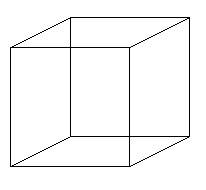
\includegraphics[scale=.7]{images/Necker_cube.png}
      \caption{The Necker Cube: insufficient sensory information to reach fixation on one explanatory model over another creates binocular rivalry between perceptual hypotheses}
        \label{fig:neckerCube}
   \end{center}
\end{figure}

It appears that human cognition has evolved a second order inferential mechanism that flexibly directs attention to certain sensory signals over others in order to successfully adjudicate between hypotheses for perceptual inputs \citep{Clark2013}.  In an inferential process likened to ``empirical Bayes,'' each error signal is conditioned with a precision weighting, which essentially functions to either ``dial-up'' or ``dial-down'' the volume on that signal's influence on the overall predictive model \citep{Clark2015}.  Precision weightings are proportional to the inverse variance of the model prior for each sensory input \citep{Ernst2004,FitzGerald2014}.  In other words, the volume of more reliable or more commonly encountered sensory inputs will be dialled-up; while the volume on less reliable or less commonly encountered sensory inputs will be dialled-down. This process of Bayesian precision weighting can be understood as the AIF's version of attention \citep{Ramstead2016}.

Precision weighting allows the brain to decide which prediction errors to pay attention to at which level of the coding hierarchy \citep[be it high and conceptual or deep and sensory][]{Friston2015}.  Iterative learning adjusts the precision weighting mechanism to strengthen prior probability distributions of models for future inference \citep{Robbins1964}.

Thus, not only does PC appear to be more computationally efficient, it also promises to be more flexible than alternative models of cognition---facilitated by a second-order mechanism of precision-weighting.  The process of prediction error minimisation accords neatly with the mandate of free energy minimisation prescribed by the AIF.  As I explain in more detail below, the PC paradigm provides a neurocomputational architecture capable of efficiently and flexibly integrating various sensory inputs (exteroceptive, interoceptive, and proprioceptive) into one overarching inferential process.


\myparagraph{Was it a thief or just the wind?\label{sect:windThief}}
To understand how the PC account applies to human cognition, consider the following example used by cognitive scientist Giovanni Pezzulo \textcite{Pezzulo2013}.  Imagine you wake up in the middle of the night to the sound of your bedroom window creaking.  At the higher levels of the predictive coding architecture, competing perceptual hypotheses emerge to explain the likely causes of the sensory experience.  For simplicity, assume that two plausible hypotheses emerge: 1) the wind outside caused the window to creak (wind), or 2) a thief is trying to break in to your house (thief).  The probability that the sensory experience of the window creaking is due to the wind can be represented by the equation in Figure ~\ref{fig:windThief}.  The predictive coding proposal is that the brain formulates a probability estimate based on:

\begin{enumerate}
  \item $P(wind)$: the model \textit{prior} formulated by previous experience (e.g., it has been windy at night recently, or in the case of $P(thief)$, there have been some recent thefts in the neighbourhood)
  \item $P(evidence|wind)$: the \textit{likelihood} that the sensory experience is caused by the wind (this value could be informed by other sources of information, e.g., the trees outside are also rustling, the dog is not barking (which may be the case if it were a thief, ($P(evidence|thief)$)
  \item Precision weighting: the reliability or certainty associated with your sensory inputs (it is dark in your room and so you may not trust your visual perception, you just woke up so could have been dreaming, etc.).  The precision weight is factored into the ``evidence.''
\end{enumerate}


\begin{figure}[htbp]
  \begin{center}
    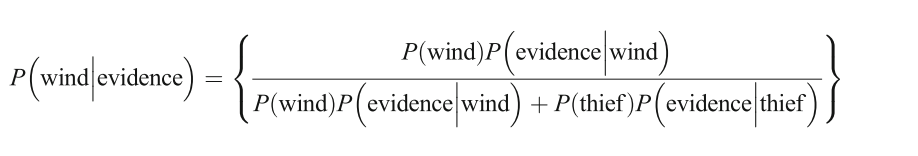
\includegraphics[scale=.5]{images/windThief.png}
      \caption{Bayesian model for the prediction of wind as the cause of the window creaking. Source: Pezzulo (2014)}
        \label{fig:windThief}
   \end{center}
\end{figure}

These two hypotheses (wind and thief) effectively compete on the basis of how well they explain the sensory stimuli.  The brain's capacity to quantify the uncertainty of any given sensory state (precision) facilitates optimal selection between competing predictions pertaining to the same bottom-up sensory signals.  In this example, based on the the priors ($P(wind) = .8$ (it has been windy recently) and $P(thief) = .2$ (no recent reports of theft)), and the (precision-weighted) evidence ($P(evidence|wind) = .6$ and $P(evidence|wind) = .5$ (roughly equivalent because it is dark and you have just woken up), the probability of wind ($= .8276$) is much higher than the probability of thief ($= .1724$).  In this case, the prediction that wind caused the window to creak wins out, and guides action and perception accordingly (you decide to go back to sleep).


\myparagraph{What makes the AIF ``active?''}
Original models of PC dealt primarily with ``exteroceptive'' information \citep[relating to stimuli that are external to an organism, i.e. visual, auditory, haptic perception][]{Rao1999,Friston2010}.  In the wind vs. thief model considered above, only exteroceptive evidence is considered, in the form of the auditory stimulus of the window creaking.  Research has since demonstrated that the PC approach can also account for ``proprioceptive'' information (relating to stimuli that are produced and perceived within an organism, especially those connected with the position and movement of the body), as well as ``interoceptive'' information  \citep[relating to stimuli produced within an organism, particularly by the body's organs (viscera) e.g., ``gut feelings,'' or elevated heart rate; see][]{Seth2013,FeldmanBarrett2015}.  Incorporating proprioceptive and interoceptive information sources into PC allows researchers to theoretically demonstrate that human cognition is both ``embodied''---inference is rooted in and contingent upon visceral, interoceptive information \citep[][]{Pezzulo2014}, as well as ``active'' \citep[in the sense that humans can move throughout the environment to reduce the discrepancy between proprioceptive predictions and actual body states, see][]{Friston2010,Clark2015}.

In the case of motor systems, agents are able to move their sensors in ways that amount to actively seeking or generating the sensory consequences that they (or rather, their predictive models) expect.  In this way, ``error signals self-suppress, not through neuronally mediated effects, but by eliciting movements that change bottom-up proprioceptive and sensory input'' \citep[][1349]{Friston2003}.  The hierarchical and nonlinear structure of predictive coding enables diverse sensory inputs feed into the same inferential mechanism.  Diverse functions of action, cognition and perception are thus integrated into an framework that is both embodied and enactive \citep{Friston2015}.  Embodied and active sources of information broaden the scope of human cognition beyond the brain and reduce reliance upon computationally intensive mental simulation as a driving force for action.  Instead, canny utilisation of extra-neural and bio-external affordances of the environment can support free energy minimisation \citep{Clark2015}.  Thus, the \textit{integrative} approach of the AIF allows for a conception of interlocking traditionally disparate sources of information---e.g., physical, emotional, and cognitive---into one inferential process.

Consider an ``active'' revision of the wind vs. thief example.  Two key differences in the model become apparent.  First, the evidence considered is broadened to include both interoceptive and proprioceptive information, in addition to exteroceptive evidence.  Assume that before you went to bed you just watched a horror movie, and when you woke up to the sound of a window creaking your heart began to pound and you immediately fixated on the hypothesis that a thief was causing your window to creak.  Fixation on the thief hypothesis can be explained by the contribution of interoceptive information (e.g., autonomic stress response, heart beat, etc.) to sensory the evidence \citep{Pezzulo2014}.  In addition, the incorporation of proprioceptive information into the model (for example, the possibility of moving to turn on the bed-side lamp) creates additional cognitive affordances through which higher level predictions could be strengthened (or free energy can be minimised).  This difference in the model demonstrates how perception, emotion, and action are functionally integrated in human cognition.

Second, broadening sensory inputs in the model also introduces the problem of differential reliability of sensory inputs.  The wind vs. thief example describes a situation in which exteroceptive information is relatively unreliable: it is dark, so visual inputs are restricted, and what you heard is unreliable because you just woke up and maybe it was part of a dream.  By contrast, interoceptive information is usually quite certain: you can be certain that your heart is pounding and that you feel unnerved.  In this particular case, interoceptive inputs may have a greater influence on the overall inference due to their reliability.  As explained above, evidence suggests that the brain deals with multiple sensory inputs via a process of ``Bayesian multisensory integration'' \citep{Ernst2004}, with the reliability of each sensory input proportional to the inverse of its variance.  In the wind vs. thief example, the interoceptive information from your body will be precision-weighted as the most reliable source, and will likely tip the balance of the model to favour the hypothesis that it is a thief.  In this case, you will move your body in a way so as to reconcile the discrepancy between proprioceptive predictions that also correspond to the thief hypothesis (and therefore also tuned to a higher volume in the model).  The result of this trajectory of action and perception may be that you act by turning on your bedside lamp \citep{Pezzulo2014}.

Thus, the combination of mutlisensory integration (of exteroceptive, proprioceptive, and interoceptive information) and Bayesian precision-weighting of prediction errors provides the necessary mechanics for a conception of human cognition that is both active and embodied.    In the following section, I introduce the concept of affordances as a necessary compliment to the PC paradigm and a core component of the AIF.

%Even if turning on the light would subsequently reveal that it was the wind all along,

%[; for a detailed discussion of the differences between traditional and active inference approaches to motor control, see Appendix ~\ref{app2:theory} Section  ~\ref{app2:motorControl}]  In the next section, I explain how active inference can be applied to joint action and shed light on the phenomenon of team click.



\subsubsection{Affordances}
In this section I introduce the concept of affordances as a necessary compliment to the generative models and its relevance to the AIF.  In brief, affordances can be understood within the AIF as extra-neural resources that couple with generative models to produce loops of action and perception \citep{Ramstead2016,Clark2015}.  The concept of affordance is crucial to facilitate an understanding how active inference unfolds in real-world settings.  While affordances have traditionally been studied narrowly as localised resources for basic perception \citep[e.g.][]{Fajen2011}, researchers working with the AIF have proposed an extension of the the concept of affordances to include a spectrum of objects, ranging from content-limited ``natural affordances,'' through to content-rich affordances mediated by cultural conventions and institutions \citep[cf.][]{Roepstorff2010,Ramstead2016}.

The theory of affordances, originally proposed by psychologist \textcite{Gibson1979} states that the world is perceived not only in terms of object shapes and spatial relationships, but also in terms of object possibilities for action.  This definition accords neatly with the propositions of the AIF, which posits Bayesian inference machines reliant on cognitive resources distributed throughout brains, bodies, and physical features of the task-specific environment in circular causal loops of perception and action.  Put simply, an affordance is the attribute of a hidden cause in the environment that induces (through PC architecture) predictions \citep[908]{Pezzulo2013}.  Repeated coupling between generative models and their extra-neural correlations in the environment give rise to dense causal relations between particular affordances and particular predictions.

Working within the AIF, \textcite[7]{Ramstead2016} propose that the extra-neural cognitive resources to which generative models couple (i.e., affordances) can be understood as a spectrum, with ``natural affordances'' at one end, and ``conventional affordances'' at the other \citep{Ramstead2016}.  Natural affordances pertain mainly to basic correlations between the organism and the environment that enable sensorimotor control and regulation: the physical features of the environment; the ground beneath our feet.  Conventional affordances, by contrast, often rely on consensus from other agents and culturally derived regularities; the carpet beneath our feet, or the keys at our fingertips, for example.  As Ramstead and colleagues explain:

\begin{quote}
  Successfully learned human conventions that govern action are also best conceptualised as affordances. Such affordances depend on shared sets of expectations, reflected in the ability to engage immersively in patterned cultural practices, which reference, depend on, or enact folk ontologies, moralities and epistemologies. We might call these ``conventional'' affordances.
\end{quote}

As \textcite[906]{Pezzulo2014} points out, PC hierarchies extend well beyond hypotheses concerning the source and reliability of immediate sensory inputs. At higher levels of the PC hierarchy, more profound regularities can be represented, such as long-term beliefs that are increasingly more removed from sensorimotor events. In humans, while higher order beliefs may be acquired mainly through cultural learning (rather than purely ``from the ground up'' via natural affordances),  these beliefs may still remain ``grounded'' through the linkage with lower-level sensory events).  Indeed, higher-order beliefs may need to remain grounded in sensory experience in order to retain long-term viability.

\textcite{Bruineberg2014} propose that affordances should be conceived of using a three-step topology. For any given agent, there exists a ``landscape'' of all possible affordances, within which an agent only engages with a specific ``field'' of affordances prescribed by the patterned coupling between predictive models and natural and cultural features of the environment; the affordances to which an individual brain is coupled at any one moment can be understood as ``solicitations.''  This three-level topology of affordances allows for a conception of the way in which repeated agent-environment coupling can give rise to particular regimes of attention, action, and perception within a vast landscape of all possible affordances.

When a specific field affordances or set of solicitations are conventional and shared, repeated coupling can generate regimes of \textit{shared} attention. For the purposes of this dissertation, conventional (cultural) affordances can thus be understood as regularities in the environment that cue multi-modal predictions for joint action.  This understanding incorporates factors that are traditionally understood to b psychologically explicit or ``external,'' such as societal values or similar cultural dimensions, \citep{Hofstede1991,Schwartz1992}, social practices and artefacts  \citep{Nisbett2003a}, as well as and ``internal,'' such as dominant modes of self-construal or dispositional and linguistic tendencies \citep{Markus1991}.  The concept of affordances enables an extension of the AIF beyond immediate sensorimotor processes, and into the domain traditionally understood as ``culture'' \citep{Roepstorff2010}.

In sum, the concept of affordances is an indispensable compliment to generative models of the AIF.  As discussed in the previous section (Section ~\ref{sect:predictiveCoding}, generative models can be understood as containing a spectrum of statistical complexity, ranging from basic (content-free) to elaborate (and seemingly content-rich) correlations.  The affordances to which these models couple (and therefore on which such models depend) can likewise be conceived of as existing on a spectrum, spanning natural and conventional (cultural) variants.  Importantly, the concept of affordances reveals the fact that higher-order generative models are contingent on couplings with higher-order affordances, i.e., culturally shared affordances.  In other words, higher cognitive processes are fundamentally social processes.   The correlation in complexity between generative models and their affordances provides a proximate explanatory mechanism for the observable fact that higher-order cognitive capacities for belief, reason, and language appear to be fundamentally contingent social and cultural processes, rather than purely innate capacities for which humans are naturally endowed \citep{Sperber1997,Henrich2015}.  The concept of affordances also offers an explanation for observable cross-cultural variation in action, perception, and attention \citep[cf.][]{Nisbett2003}.  Selective engagement with specific fields of affordances give rise to regimes of shared attention and beliefs that direct trajectories for individual and collective activity.


\myparagraph{Summary of the active inference approach to joint action}
To summarise, the AIF entails a radical inverse of traditional models of cognition that rely predominantly on bottom-up sensory inputs and top-down feature detection \citep[e.g.,][]{Marr1985}. Instead, active inference posits that top-down predictive models themselves shape perception and action, and the only information that travels forward (or from the ``bottom-up'') is the error signals that arise from discrepancies between predictions and the sensorium \citep{Pickering2014}.  AIF depicts a human cognitive system in which perception, mental simulation, emotion, and action are functionally and temporally integrated to manage uncertainty (free energy) inherent in interactions with the environment \citep{Clark2013}.  Importantly, these processes of generative modelling are dynamically coupled with affordances that span a spectrum of basal natural correlations with the physical features of the environment, through to elaborate culturally mediated beliefs and conventions.  The integrative approach of AIF allows for a theorisation of the interlocking physical, affective, and social dimensions of group exercise.


\section{Active inference applied to joint action \label{sect:activeInfJA}}
As explained above, traditional theoretical models of human cognition have struggled to integrate cognition with emotion, mental simulation with habitual response, flexibility with efficiency \citep{Clark2015}.
Team click is a powerful subjective experience in which many of these binaries appear to collapse and co-occur.  The AIF approach promises a testable theory of the embodied and dynamic dimensions of joint action.  In this section, I outline existing attempts to apply the AIF to joint action, and point to predictions relevant to team click and social bonding in joint action.
%, which appear to be maximised in team click.

%\myparagraph{Auxiliary approaches to joint action}
The AIF proposal offers a more integrative alternative to existing models of joint action, which rely on mechanisms of sensory prediction (of self, other, and joint actions) that are individually-bounded and auxiliary to joint action itself \citep{Pesquita2017}.   \textcite{Keller2016}, for example, presented a conceptual framework that applies an ``auxiliary forward model'' (AFM) approach to musical joint actions.  The AFM approach requires that agents produce predictive models responsible for individual action planning and control (self-internal models), prediction of others' actions (other-internal models), and representation of the shared goal (joint-internal models).  Of these three types of models, however, only self-internal models comprise the auxiliary predictive architecture (i.e., the forward model containing an efference copy of one's own action, and ``inverse models'' that are responsible for output of motor commands ~\ref{app2:theory}, Section ~\ref{app2:motorControl} for a more detailed explanation of these terms).  Thus, both anticipation and compensation in joint action depends on a control loop, whereby sensory information (error signals) are routed (fed-back) through self-internal models, which inform the production of auxiliary predictions---of self, other, and joint action---grounded in individual motor simulations.  Importantly, in this model,  error signals are fed-back only to the self-inverse model, as no inverse model for the joint action partner exists.

The now longstanding proposal that individuals only produce auxiliary predictive models of their own actions (as opposed to others' actions too) has served to explain how individuals effectively attend to others in joint action.  With privileged access to an efferent copy of impending individual action, an agent is able to preemptively attenuate sensitivity to their own action, in order to attend to the actions (and prediction errors) of others \citep{Wolpert1998}.  For example, the AFM approach provides an explanation for the phenomenon of tickling, or specifically why it is near impossible to tickle oneself \citep[due to sensory attenuation resulting from the self-generated predictions about the consequences of action][]{Blakemore2003}. However, while the AFM has proven adequate to explain individual motor control, and some instances of joint action (such as tickling), it also contains potential shortcomings when applied to dynamical joint action scenarios.

\textcite{Pesquita2017} summarise three shortcomings when applying AFM to joint action.  First, the AFM model assumes a static and unchanging representation of the shared goal and the other's goal, and provides no mechanism through which the shared goal representation can be dynamically updated (based on prediction error signals).  This issue limits the ability of AFM to account for the real-world flexibility and interchangeability of shared goals (for example, the adaptive switching between the shared goal of carrying a table or the bench depending on the location of both objects).  Second, the same rigidity applies to other-inverse models.  The inability to directly and dynamically update other-models suggests the practical possibility that self and other models may gradually diverge over time due to the lack of sufficient predictive information regarding the actions of others \citep{Pickering2014}. Third, the AFM approach does not specify how sensory input is differentially used to update self and other models, which limits the model's ability to account for learning and adaptation within joint action \citep{Pesquita2017}.  Thus, not only does the AFM approach appear to be computationally intensive (due to the recruitment of auxiliary inverse models and dual motor commands, discussed in Section ~\ref{sect:predictiveCoding}), it also appears to be unable to fully account for the dynamic flexibility of real-world joint action.

\myparagraph{Generalised synchronisation as a dynamical foundation for joint action}
The AIF offers a thoroughly dynamical approach to joint action, whereby two (or more) Bayesian predictive brains committed to modelling each other in order to minimise free energy \citep{Friston2015,Friston2015a}. In order to achieve free energy minimisation, the sensory stimuli produced by co-actors in joint action must be pre-emptively modelled, just like other features of the sensorium (as explained above, see Section ~\ref{sect:thermoCog}).  This necessitates a scenario in which brain A has a model of brain B, which includes the fact brain B is modelling brain A, and so on---\textit{ad infinitum}.

The recurrent predictions of both brains about one another threatens an infinite runaway regress that could preclude accurate modelling of either brain.  However, as Friston and Frith demonstrate formally (mathematically), this recursion dissolves if the models of the two brains are formally similar \citep{Friston2015}.  When grounded in computational similarity, each brain is able to generate predictions of the sensory outcomes caused by itself and the other in the same way.  The authors propose that this will lead to dynamical ``generalised synchronisation'' \citep{Barreto2003}, or dynamical coupling between the internal models of both brains (for a more detailed explanation of general synchronisation and its dynamical underpinnings, see Appendix ~\ref{app2:theory} Section ~\ref{sect:generalSync}).  In this way, two or more brains are able to accurately predict each other's behaviour based on feedback of exteroceptive (sensory information from the actions of others and the task environment) and proprioceptive (pertaining one's own contribution to joint action) prediction errors.  In essence, other agents exist as affordances to which individual brains couple, and upon which individual brains become dependent for ongoing (joint) processes of action, perception, and attention.

In place of auxiliary processes of prediction, the AIF for joint action hinges instead on precision weighting of prediction errors in order to facilitate and finesse joint action \citep{Friston2015}.    When engaged in joint action, the individual turns down the volume (reduce the precision weighting) on prediction errors relating to one's own action so that movement can occur unimpeded by over-attention to self-generated prediction errors \citep[an intuitive example of the opposite of this ideal scenario is a Skype call in which the flow of an individual's speech is interrupted by auditory feedback from the other receiver's device (feedback that would otherwise be attenuated by the speaker), see][]{Friston2015}.  Alternatively, when attending the the action of others, the attenuation of proprioceptive error signals can cease. In this way, precision weighting is used to flexibly adjust the volume of multi-modal prediction errors (exteroceptive, interoceptive, and proprioceptive) in order to finesse and sustain generalised synchronisation---the shared narrative on which joint action is sustained).

Heuristically, this suggests that active inference in joint action takes one of two modes; either 1) flexibly attending to sensations or
2) acting during periods of sensory attenuation \citep{Friston2015}.  The active inference explanation for ticklishness, for example, is an inferential mode in which the volume on proprioceptive prediction error is ``dialled-up.''  The failure of self-tickling, by contrast, pertains to a mode of active inference in which the volume of proprioceptive prediction is ``dialled-down'' to enable smooth flow of action execution.
  \footnote{Recall also that instances of tickling commonly involve a stationary victim. While it indeed appears almost impossible to tickle oneself, it is also rare to be tickled while moving, i.e., acting during periods of sensory attenuation.}


\myparagraph{Predictive Joint Action Model (PJAM)\label{sect:PJAM}}
\textcite{Pesquita2017} have formulated a minimal architecture for an active inference approach to joint action, which they term a ``Predictive Joint Action Model'' (PJAM).  PJAM is comprised of three hierarchical levels of inference: goal representation, action-planning, and sensory routing (see figure ~\ref{fig:PJAM}).  Each level of the hierarchical model is informed by prediction errors from the level below, and the model works iteratively to minimise free energy in joint action scenarios.  In line with the AIF, PJAM does away with auxiliary processes of motor control and efferent copies, and posits instead that joint action emerges directly from two or more individuals reaching generalised synchronisation by converging on equivalent predictive models for joint action \citep{Friston2015}.

  \begin{figure}[htbp]
    \begin{center}
      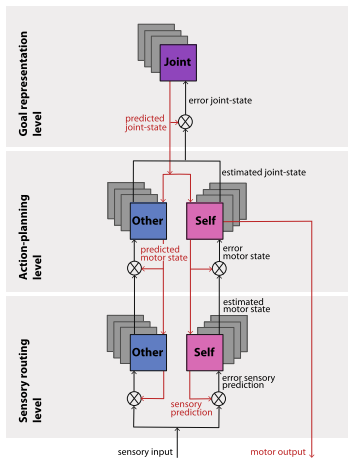
\includegraphics[scale=.8]{images/PJAM.png}
        \caption{The Predictive Joint Action Model \citep{Pesquita2017}}
          \label{fig:PJAM}
     \end{center}
  \end{figure}

In contrast to the AFM approach, which posits a shared goal representation deriving from self-internal models, the PJAM suggests that a shared goal derives primarily from the dynamical coupling of agents to each other and to other (shared) affordances of the task-specific environment.  Thus, rather than being wholly explicit, propositional, or pre-set, the shared goal is understood to span the entire predictive hierarchy, with basal coupling of sensorimotor processes at the lower end, through to more elaborate models that facilitate more explicit or propositional content, at the higher end.  In a bidirectional cascade of prediction and prediction error, the ``shared narrative'' at the goal representation level generates discrete action plans for self and other, which are then tested against prediction errors arising from the sensory routing models below \citep{Pesquita2017}.


\subsubsection{Evidence in support of PJAM}
PJAM (and the AIF which it extends) predicts that joint action will be established and maintained through generalised synchronisation between two or more predictive brains driven by an overarching mandate of free energy minimisation \citep{Friston2015}.  In particular, PJAM predicts that co-actors in joint action will generate predictive models that reflect 1) a shared goal, 2) action plans for self and other, and 3) routing instructions for sensory inputs.  Consistent with the modelling view of the AIF (see Section ~\ref{sect:thermoCog}), these three layers of generative models will reflect an hierarchy of complexity, and will be coupled to a continuum of natural and conventional affordances.  Below I outline existing experimental evidence in support of these predictions.

\myparagraph{Evidence for generalised synchronisation in joint action}
Evidence that musicians maintain shared representation of desired unified sound of an ensemble \citep{Keller2008}, track deviations from desired joint state \citep{Loehr2013}, and allow shared goal predictions to guide future action \citep{Loehr2016}, confirms the hypothesis that co-actors share a dynamical and flexible shared goal---a shared narrative or common ground.  PJAM specifically predicts that the foundation for this shared narrative will be dynamical, i.e., it will involve coupling of system component degrees of freedom of co-actors in joint action \citep{Turvey1978,Schmidt1990}. Dynamic coupling can be identified by two core properties:  1) dimensional compression (potentially independent DF are coupled so that the synergy possesses a lower dimensionality than the set of components from which it arises) and 2) reciprocal compensation \citep[the ability of one component of a synergy to react to changes in others][]{Riley2011}.

An accumulation of evidence on multiple levels of human behaviour, from brain function \citep{Yufik1998,Sengupta2013}, to interpersonal interactions \citep{Kelso2009,Riley2011,Fusaroli2014}, to large-scale human societal dynamics \citep{Nowak2017} supports the existence of dynamic coupling.  In the case of joint action in particular, individuals have been found to couple and reciprocally constrain their movements reducing the overall control needed to maintain effective cooperation \citep{Ramenzoni2011,Ramenzoni2012,Riley2011,Schmidt1990}.  Studies of real-world joint action scenarios such as dancing, martial arts, and moving objects like furniture have revealed evidence for dynamic coupling between co-actors.  In these studies, specific component degrees of freedom are modelled as coupled oscillators \citep[using the HKB model, which describes the change in the relative phase between two oscillatory components. See][]{Haken1985,Kelso1986}.  Interestingly, dynamic coupling of movement has been measured beyond dyadic synchronisation, in the analysis of sub-phases of team sports \citep{Passos2014,Duarte2012} and group dancing \citep{Chauvigne2017}.  For a more thorough explanation of dynamic coupling in human movement systems, including methods for measuring dynamical quantities, see Appendix ~\ref{app2:theory} Section ~\ref{app2:dynamicCoupling}.

This evidence is supported by recent research focussed on the movement signatures of joint action that resemble instances of ``identical synchronisation,'' or the idea of being ``in the zone'' with a co-actor. Working within the common dyadic ``mirror game'' paradigm, \textcite{Noy2011,Noy2015,Hart2014} have identified ``co-confident motion'' (CC motion) as a canonical movement pattern of synchronised motion characterised by smooth and jitter-less motion, without the typical jitter resulting from reactive control in more commonly encountered leader-follower patterns.  In CC motion, different players appear to shift their basic motion signatures to a movement shape that is altogether different from their individually preferred shapes \citep{Hart2014}. Importantly, the pattern of CC motion shares the same sine wave shape as the optimal solution of the minimum jerk model, a well-known motor control model for rhythmic motion \citep{Hogan2007}.  This evidence accords with the proposal that joint action is underwritten by a ``shared narrative'' that transcends individual action tendencies of self and other and produces a  ``we-mode'' of social cognition (exemplified by CC motion) \citep{Gallotti2013}.

\myparagraph{Evidence for self and other action plans}
On the level of self and other action plans, experimental evidence suggests that co-actors generate internal models of self and other either spontaneously and involuntarily---as in the commonly used social simon task experimental paradigm \citep{Sebanz2003,Atmaca2008}---or more deliberately---as in a coordinated dyadic horizontal jumping task \citep{Vesper2012}.  \textcite{Loehr2016} demonstrate that when learning a joint piano piece, musicians are able to better perform a piece together rather than solo, which suggests that representations about each participant in joint action are encoded within the joint context of the interaction.  Studies also show that the capacity for co-representation of self and other action plans is modulated by mood \citep[positive or negative affect, see][]{Kuhbandner2010}, self-concept and social orientation \citep{Colzato2012,Colzato2012a}, and processes of group membership \citep{DeBruijn2008,Iani2013}. This evidence lends support to the proposal that active inference involves coupling with various natural and conventional affordances in order to flexibly integrate information deriving form various sensory inputs.

The evidence outline immediately above is supported by parallel strands of research in psychology \citep{Prinz1990,Prinz1997,Prinz2013}, neurophysiology \citep{Rizzolatti2004,Rizzolatti2010}, and neurocognition \citep{Wolpert1998,Wolpert2000} that interpersonal behavioural coordination in joint action is facilitated by the intrinsic links between action perception and action execution in the human brain.  In essence, action-perception coupling refers to the ostensive co-occurrence of a stimulus for action and its motor representation.  For example, for individuals who have mastered a certain sensorimotor task, the representation of a perceptual effect (say the sound of a middle-C on a piano) can trigger the movement necessary to produce the effect itself (motor instructions for playing the middle-C key on a piano) \citep{Novembre2014}. Evidence suggests that skilled individuals not only develop generative models for self action, but also for the actions of others in joint action \citep{Novembre2012}. Action-perception links can be used for monitoring and integrating (e.g., timing or combined pitches) the actions of other ensemble members with self-generated actions \citep{Loehr2013}, and these effects appear to be stronger in individuals with high perspective taking skills \citep{Novembre2012,Loehr2013}.  The overlap between mechanisms for action production and action observation suggests that individuals may represent their own and others’ actions in a commensurable format.  Training-induced motoric representation of self and other actions may facilitate various capacities important for joint action, such as prediction, adaptation, and entrainment (for a more detailed treatment of action-perception links and their relevance to joint action, see Appendix ~\ref{app2:theory} Section ~\ref{app2:actionPerceptionLinks}).

\myparagraph{Evidence for sensory routing}
On a sensory-routing level, evidence suggests that modulation in sensory attenuation is driven by the predictability of the outcome, as opposed to necessarily being driven by the presence or absence of auxilliary efference copies \citep{Sato2008}.  In addition, attributing sensory consequences to joint action partners is linked to cooperative success \citep{Chaminade2012}, suggesting that finely tuned sensory routing based on predictions of self and other actions could be key to successful coordination.

In sum, PJAM provides a framework for the function of active inference in joint action.  PJAM proposes a dynamical model of joint action, whereby the predictive models of two or more brains are coupled to produce a common ground upon which free energy minimisation can occur.  In the section below, I outline how this process of general synchronisation could explain the phenomenon of team click, as well as the achievement of social connection through joint action.



\subsection{AIF for team click and social bonding in joint action\label{sect:AIFclickBonding}}

How can the AIF be used to account for team click and social bonding in joint action? In this section, I draw attention to evidence for mechanisms relevant to joint action that could generate

As explained in Chapter~\ref{chap:intro}, the link between joint action and social bonding has been addressed in the behavioural mimicry and synchrony literatures (see Chapter~\ref{chap:intro} Section ~\ref{sect:socialHigh}).  There is now strong evidence to suggest that a combination of 1) neuropharmacological reward arising from lower-cognitive affective mechanisms \citep[see][]{Mogan2017},, 2) self-other merging resulting from neurocognitive alignment \citep{Rizzolatti2010}, and 3) reinforcement of cooperative relationships owing to experience of interpersonal association in joint action \citep{Reddish2013} generates a psychophysiological environment conducive to generating social bonds.  Yet, almost all of these studies operationalise joint action as exact in-phase behavioural synchrony, and there is much less substantive evidence of the bonding effects of complex and dynamic joint action scenarios \citep[but see][]{Marsh2009,Miles2009,Lumsden2012}.



Secondly, and more fundamentally, research dedicated to the putative synchrony-bonding link focusses most of its attention on the proximate and affective mechanisms of joint action, and accounts less for how synchrony-induced lower-level physiological and affective mechanisms facilitate higher-order cognitive and social processes associated with bondedness, social cohesion, and cultural transmission \citep{Heyes2012}.

As I argue in this dissertation, these dual shortcomings of the social cognition of joint action represent two sides of the same coin. On one side, how behaviourally complex joint actions generate social and physiological effects remains poorly theorised; on the other side, the causal role of physiological and social effects on complex cognitive and cultural processes (i.e., cultural transmission and evolution) is also poorly understood.  I suggest that adopting an integrative model of cognition (the AIF) can help advance understandings of the interlocking physical, affective, cognitive, and cultural mechanisms of social connection in joint action and cognitive and evolutionary processes more generally \citep{Ramstead2018}. Indeed, the AIF serves to collapse the traditional proximate-level distinction between physical, affective, cognitive, and cultural processes, under one overarching mandate of free energy minimisation.

\subsubsection{Team click}
As discussed above, the AIF for joint action, summarised in PJAM above, suggests that successful performance and social connection in joint action require not just exact behavioural synchrony, but generalised synchronisation of two or more free energy minimising systems \citep{Friston2015}.  Dynamical coupling of cognitive processes entails a continuum of generative models within brains tightly coupled to a spectrum of natural and conventional affordances---specifically the affordances of co-actors, but also other features of the neuro-external environment \citep{Clark2015}.

Considered from the perspective of the AIF, the experience of team click and social connection in joint action will derive not simply from exact coupling of sensorimotor processes (as in the case of behavioural synchrony), or else to more explicitly perceived alignment of shared expectations surrounding a joint task \citep[cf.][]{VanderWel2012}.
Rather, the click of joint action will theoretically entail an entire double helix of interlocking predictions and affordances spanning the most basic correlational models of sensorimotor coupling, through to the most densely semantic and proposition forms of explicit knowledge and communication.

In this section I reduce the components of team click outlined above to three core dimensions---surprise, viscerality, and agency---for which the mechanisms of the AIF can offer predictions (see Table ~\ref{tab:teamClickMechanismsAIF}).  The relevant mechanisms of the AIF are predominantly associated with processes of second-order Bayesian inference, specifically affective reward mechanisms associated with ``exploitation-exploration'' dynamics in free energy minimisation \citep{Friston2012,Schwartenbeck2013,FitzGerald2014,Chetverikov2016}, 2) reliability-based multi-modal sensory integration \citep{Ernst2004}, and 3) flexible attenuation ~\citep{Frith2007,Friston2015} of exteroceptive and proprioceptive inputs in dynamic joint action.  In brief, the affective, visceral, and agentic dimensions of team click suggest that team click sets the foundation for social bonding, which I propose here to include elements of emotional support and perceptions of common goal \citep[cf.][]{Dunbar2012,Wolf2015}, as well as shared social identity between co-actors \citep{Whitehouse2014}.  I review each dimension of team click below and propose relevant mechanisms of the AIF.

% Please add the following required packages to your document preamble:
% \usepackage{booktabs}
% \usepackage[normalem]{ulem}
% \useunder{\uline}{\ul}{}

\newpage
\newgeometry{margin=0.5cm} % modify this if you need even more space
\begin{landscape}

\begin{table}[]
\begin{tabular}{@{}lllll@{}}
\toprule
\textbf{Component}                                                        & \textbf{Dimension} & \textbf{AIF mechanism}                                                                                        & \textbf{Predicted function}                                                                                                                                                                                                                                                                                                                                                                                                                & \textbf{Predictions for joint action}                                                                                                                                                                                                                                      \\ \midrule
Surprise                                                                  & \textbf{Affective} & \begin{tabular}[c]{@{}l@{}}Precision-weighting \\ (exploitation exploration, \\ cf. Friston2013)\end{tabular} & \begin{tabular}[c]{@{}l@{}}Attention will be allocated to sensory inputs\\  as a function of their prior probability\\ distribution; Affect (surprise) will\\  be allocated to predictions as function of inverse \\ prior probability; i.e., higher probability predictions \\ receive more attention but lower reward; lower probability predictions \\ but receive less attention but higher \\ reward (Chetkerov, Fiston)\end{tabular} & \begin{tabular}[c]{@{}l@{}}Inherent uncertainty of real-world joint action \\ (the df problem, cf. Bernstein 1967), makes successful coordination improbable, but highly rewarding:\end{tabular}                                                                           \\
                                                                          &                    &                                                                                                               &                                                                                                                                                                                                                                                                                                                                                                                                                                            &                                                                                                                                                                                                                                                                            \\
Group flow                                                                & \textbf{Visceral}  & \begin{tabular}[c]{@{}l@{}}Multimodal sensory integration \\ (Pezzulo 2014)\end{tabular}                      & \begin{tabular}[c]{@{}l@{}}More reliable sensory inputs will receive greater \\ precision-weighting\end{tabular}                                                                                                                                                                                                                                                                                                                           & \begin{tabular}[c]{@{}l@{}}Unreliability of exteroceptive predictions in joint \\ action will generate a decrease precision \\ on exteroceptive predictions, and increase precision of\\ interoceptive predictions (Pezzulo2014,\\ Seth2013, Feldman Barrett)\end{tabular} \\
                                                                          &                    &                                                                                                               &                                                                                                                                                                                                                                                                                                                                                                                                                                            &                                                                                                                                                                                                                                                                            \\
Tacit understanding                                                       &                    &                                                                                                               &                                                                                                                                                                                                                                                                                                                                                                                                                                            &                                                                                                                                                                                                                                                                            \\
                                                                          &                    &                                                                                                               &                                                                                                                                                                                                                                                                                                                                                                                                                                            &                                                                                                                                                                                                                                                                            \\
Atmosphere or aura                                                        &                    &                                                                                                               &                                                                                                                                                                                                                                                                                                                                                                                                                                            &                                                                                                                                                                                                                                                                            \\
                                                                          &                    &                                                                                                               &                                                                                                                                                                                                                                                                                                                                                                                                                                            &                                                                                                                                                                                                                                                                            \\
\begin{tabular}[c]{@{}l@{}}Blurred self and other \\ agency\end{tabular}  & \textbf{Agentic}   & Sensory attenuation                                                                                           &                                                                                                                                                                                                                                                                                                                                                                                                                                            &                                                                                                                                                                                                                                                                            \\
\textit{}                                                                 &                    & Precision-weighting                                                                                           &                                                                                                                                                                                                                                                                                                                                                                                                                                            &                                                                                                                                                                                                                                                                            \\
\begin{tabular}[c]{@{}l@{}}Ability extended \\ by others\end{tabular}     &                    &                                                                                                               &                                                                                                                                                                                                                                                                                                                                                                                                                                            &                                                                                                                                                                                                                                                                            \\
\textit{}                                                                 &                    &                                                                                                               &                                                                                                                                                                                                                                                                                                                                                                                                                                            &                                                                                                                                                                                                                                                                            \\
\begin{tabular}[c]{@{}l@{}}Reliability of self \\ and others\end{tabular} &                    &                                                                                                               &                                                                                                                                                                                                                                                                                                                                                                                                                                            &                                                                                                                                                                                                                                                                            \\
                                                                          &                    &                                                                                                               &                                                                                                                                                                                                                                                                                                                                                                                                                                            &                                                                                                                                                                                                                                                                            \\ \bottomrule
\end{tabular}
\caption{Dimensions of team click and their relevant mechanisms as predicted by the AIF.}
\label{tab:teamClickMechanismsAIF}
\end{table}

\end{landscape}
\restoregeometry


\myparagraph{Surprise or positive violation of expectations in performance\label{sect:surprise}}

As explained in Section ~\ref{sect:teamClickIntro}, team click in joint action is associated with strong positive affect: pleasurable, autotelic sensations of rush or flow.  While optimal performance in joint action is perhaps always the ultimate goal, particularly for elite practitioners such as athletes and music or dance performers, when team click occurs it also often appears to be unanticipated and surprising.  Thus, team click is experienced as a \textit{positive} violation of expectations around team performance.

Surprise is a term with various connotations on different levels of analysis.  As an emotion, surprise can generally take one of two forms according to its affective valence, i.e., surprise that carries a positive valence (as in the case of team click, for example) or surprise that carries a negative valence  \citep[in the case of shock or fright][]{Chetverikov2014}.  The affective experience of surprise thus appear to be linked with cognitive processes of prediction, specifically the experiential manifestation of discrepancy between a predicted state and an actual state \citep{Foster2015}.  The precise details of this link, are yet to be fully understood, however \citep{Schwartenbeck2013}.

Considered from the point of view of traditional predictive (forward) models of cognition (such as the AFM, see Section X), negatively valenced surprise makes sense, at least intuitively.  If the brain is
in the business of reducing the discrepancy between predicted and actual states, then negative surprise will act as a signal to motivate a reduction in prediction errors.  However, this intuition leaves less room for an understanding of positive surprise.  If the goal is to reduce prediction error, why would surprise be rewarded with such powerful sensation?

The puzzle of positive surprise relates to a more general paradox associated predictive forward model approaches to cognition, described as the ``dark room dilemma'' \citep{Mumford1992}.  As evocatively described by Mumford:

      \begin{quote}
        How can a neural imperative to minimise prediction error by enslaving perception, action, and attention accommodate the obvious fact that animals don’t simply seek a nice dark room and stay in it? Surely staying still inside a darkened room would afford easy and nigh-perfect prediction of our own unfolding neural states? Doesn’t the story thus leave out much that really matters for adaptive success: things like boredom, curiosity, play, exploration, foraging, and the thrill of the hunt? \citep[243]{Mumford1992}
      \end{quote}

Although it is readily observable that animals live in a changing and challenging world and deploy quite complex strategies to survive and thrive within diverse and dynamic environments, original forward models lacked a sufficient theoretical justification for why the predictive drive did not simply lead to dark room stasis \citep{Clark2013}.  Encased within traditional linear and passive stimulus-response models of cognition, an account of co-existing and competing drives for familiarity and novelty proved difficult \citep{Kelso2009}.

However, when considered from within the unifying framework of free energy minimisation, the dark room dilemma dissolves, and the role of positive surprise becomes clearer.  As the free energy principle states, every system that maintains itself conforms to the imperative of minimising the surprise associated with the states it encounters \citep{Friston}.  Surprise is defined here in an information-theoretic sense as an approximation of average free energy, rather than necessarily an affective experience \citep[in fact, Tribus distinguished information-theoretic ``surprisal'' from surprise in an active attempt to separate the two concepts cf.][]{Tribus1961}.  Within the AIF, minimisation of surprisal exists on two scales: minimisation of long-term surprisal of the organism (i.e., entropy), as well as minimisation of surprisal in a given generative model \citep[i.e., free energy, see][2]{Schwartenbeck2013}.  Given the complex and hierarchical structure of generative models, which exist across multiple timescales and sensory modalities,  minimising surprisal in the context of one model may generate surprise in the context of another model.  The free energy principle thus explains why humans, far from being bound to seek out a dark room, are instead compelled to minimise free energy at multiple scales via co-existing strategies of ``exploitation'' (optimal free energy minimisation of a specific generative model), and ``exploration'' \citep[optimal free energy reduction of surprisal on broader scales, i.e., in the context of other generative models or the life of the organism more generally; see][]{Cohen2007}.  As Clark explains,

      \begin{quote}
        Change, motion, exploration, and search are themselves valuable for organisms living in worlds where resources are unevenly spread and new threats and opportunities continuously arise.  This means that change, motion, exploration, and search themselves become predicted and enacted accordingly \citep[193]{Clark2013}
      \end{quote}

Thus, while it is plausible that the emotion of surprise is somehow tethered to cognitive processes of prediction error minimisation, the AIF demonstrates that this relationship does not align in a 1:1 fashion, and instead is governed by the overarching mandate of free energy minimisation.  As such, the emotional experience of surprise could conceivably span a full spectrum of positive and negative of emotional valence, depending on the location of surprisal in various generative models.  In the case of team click, for example, positive surprise could arise form a scenario in which an individual is fixated on the exploitation of a specific generative model (for example, focus on individual movement), and this model is violated (surprisal) by the less anticipated successful joint action.

Researchers have hypothesised that exploitation-exploration dynamics are supported by a relationship between second-order Bayesian inference (precision weighting) and affective reward  \citep{Friston2012,Chetverikov2016}.  First, precision (attention) will be assigned to error signals as an inverse function of the variance of their prior probability distribution.  In other words, if a prediction pertaining to a sensory input is highly likely (based on prior experiences), then the variance of its prior probability distribution will be low (positive kurtosis) and it will receive greater precision weighting.  Second, affective reward will be assigned to error signals as a direct (as opposed to inverse) function of the variance of their prior probability distribution. In essence, the less likely a prediction is to be correct, the more surprise (in an affective sense) it will entail.  Thus, while highly predictable inputs will receive a certain amount of affective reward, reward will diminish as unfolding action consumes the gradient of free energy, producing a spiky, less attractive reward.  Meanwhile, scenarios involving highly variable prior probability distributions, such as dynamic coordination of behaviour in joint action, promise powerful affective payoffs.

Neurobiological evidence generally supports this proposal, however it is yet to be thoroughly tested empirically.  Cortical processes of prediction error management appear to be mediated by the activity of the dopaminergic system \citep{Kakade2002,Schultz2016}, while subcortical neuromodulatory systems, such as those responsible for producing norepinephrine, acetylcholine, and endogenous opioids, appear to be involved in attuning cortical processing to signals from the body and environment that are important for survival \citep{Lewis2005}.

In sum, positive violation of expectation in joint action could pertain to the momentary transfer of attention away from more reliable inputs (such as the sensorium most proximate and controllable by an individual) towards sensory inputs deriving from dynamic general synchronisation.


\myparagraph{Viscerality}
The second dimension of team click is its viscerality, expressed in the components of group flow, tacit understanding, and team atmosphere.  The experience of team click is rooted in the body as something that is felt.  While not always able to articulate the sources of team click, athletes develop a fine-grained sensitivity for it; a gut feeling, or intuition.  What mechanisms are capable of exaplaining how an intricately complex cognitive phenomenon such as team click comes to be experienced primarily as a feeling rooted in physicality?

As with the phenomenon of (positive) surprise, the AIF offers a mechanistic explanation of viscerality in joint action, based on the process of Bayesian multisensory integration \citep{Ernst2004}.  As explained in the wind vs thief example (see Section ~\ref{sect:windThief}), sensory evidence is weighted according to its reliability, judged probabilistically based on past experience.  It is intuitively plausible that for a Bayesian brain a dark bedroom in the middle of the night, the most immediately reliable sensory inputs will be those most accessible to the central nervous system; visual and auditory (i.e., exteroceptive) inputs will be comparatively unreliable and will be precision weighted as such \citep{Pezzulo2014}.  In some ways, exteroceptive sensory inputs in joint action reflect an analogous reliability issue \citep{Sebanz2009}. Individuals in joint action, while often dynamically coupled to one or more other co-actors in generalised synchronisation of some form, nonetheless face the challenge of modelling the various df of the task-specific movement system, which belong predominantly to autonomous agents capable of deviating at any moment---either accidently or deliberately---from the dynamical common ground of joint action \citep{Keller2016}.  The prior probability distributions of exteroceptivee predictions in joint action will therefore entail high variances, and accordingly attention will be assigned instead to interoceptive and proprioceptive inputs \citep{Seth2013}.  Consider too that active movement in joint action necessitates attenuation of proprioceptive inputs in order to enable smooth uninterrupted action ~\cite{Dietrich2004a,Friston2015}.  Thus, the AIF predicts that interoception will function as the primary inferential affordance for dynamic joint action; phenomena such as team click will be grounded in the body---as (gut) feelings and tacit understandings---owing to the relative reliability of these inputs in joint action scenarios defined by high uncertainty.

In sum, the AIF predicts that the variance of (exteroceptive) prediction error in joint action will generate a high affective payoff when joint action clicks (surprise).  Second, the intricate achievement of click in joint action will be grounded in the body, owing to its relative reliability as an affordance for active, free energy minimising inference (viscerality).  In the next section, I discuss evidence for the agentic dimension of team click.

\myparagraph{Agency}
The agentic quality of team click is identifiable in components of experience that include: blurring of boundaries between self and other agency, the feeling that one's agency is extended by the contributions of others, and the perceived reliability of others and self to contribute effective execution of joint action (see Table ~\ref{tab:teamClickMechanismsAIF}).  When the team clicks, you and I become ``we'' (blurring), thereby you extend my ability beyond that which I could achieve alone (extension), and I experience certainty about the mine and your capacity to contribute effectively to joint action execution (reliability).  What mechanisms enable blurring, extension, and reliability of agency in joint action?

Generally, research of agency in (joint) action has focussed primarily on understanding circumstances in which people 1) experience agency over actions they do not produce themselves, or else 2) fail to experience agency over actions they do in fact cause \citep[see][]{VanderWel2012}.  Research using the theory of auxiliary forward models has established evidence for a strong correlation between attenuation of proprioception and experiences of self agency \citep{Wolpert2003,Sato2008}, as well as an inverse correlation between sensory attenuation and ascribing agency to sources external to the self \citep{Brown2013}.  As has been well documented in the case of schizophrenia, attribution of agency in social interaction may be modulated by individual variation in ``locus of control'' (the degree to which events are perceived to result from one’s own actions or not), and this may be related to improper function of the parietal cortex \citep{Frith2000}. In healthy adult populations of humans, meanwhile, \textcite{Sato2008} and colleagues suggest that discrepancy between prediction and sensory input can alter the experience of agency:  unpredicted sensory input can lead to ascribing agency for that input to an external source, for example, other participants in joint action or the external environment \citep{Sato2005,Frith2007}.

Empirical evidence addressing the question of how people experience agency in actions they intentionally produce in coordination with others is less abundant \citep[but see][]{VanderWel2012,VanderWel2013}.  Perception of agency in action has been formally defined as requiring the following conditions: 1) priority (whether the intention of action precedes the action), 2) consistency between the action and the original intention, and 3) exclusivity of explanations for the cause of the action \citep{Wegner1999}.  Current evidence suggests that perceptions of self agency in joint action may be most contingent on ``consistency'' (more so that priority and exclusivity) between predictions and prediction errors along a continuum of sensorimotor and higher order perceptual models \citep[see][]{VanderWel2012}.  van der Wel and colleagues, for example, show that perceptions of agency do not decrease when an individual transfers from performing a solo action to performing the same action with a partner (thus challenging the condition of exclusivity).  Individuals do however experience a boost in agency when they transfer from performing a joint action to the same action solo, suggesting that this transfer may induce enhanced consistency owing to the greater reliability of predictions pertaining to action that is individually controlled.

Together, this evidence accords with predictions from the AIF that agency in joint action will be most reliant on the condition of consistency, particularly when there is consistency between predictions pertaining to individual contributions to joint action and their (more reliable) prediction errors.  For the AIF, exclusivity should not be a necessary condition for perceptions of agency, as long as sensory routing between self and other(s) is effectively controlled by mechanisms of Bayesian precision-weighting \citep{Pesquita2017}.  Friston and Frith propose two heuristic modes of active inference in joint action: one in which proprioception is attenuated (agentic), and one in which individuals attend to the entire sensorium.

These heuristic modes of active inherence in joint action are based on models of dyadic joint action involving turn taking \citep[i.e., in bird song exchanges][]{Friston2015}.  Dynamic joint action, by contrast, requires continual on-line execution of movement, contemporaneous with the movement of others.  The AIF currently predicts that the volume on agency-correlated proprioceptive error signals will be turned down low while participants are executing movement, and otherwise will be held at locally optimal levels for attention to the movement of others.  The co-occurence between self and other movement could generate a conflict between processes of sensory attenuation, such that an individual is forced to sustain proprioception in dynamic joint action. This situation could  thus result in a blurring of the sense of self and other agency.  Indeed, it is plausible to predict that a tradeoff or middle ground between these two heuristic modes will be optimised in dynamic joint action scenarios. Thus, it can be predicted that such scenarios will be conducive to blurring of self and other agency (blurring).  In turn, in scenarios in which the boundaries of agency are blurred, attention to the contribution (and reliability of contribution) to joint action by others will be increased, and iteratively strengthened with repeated experiences of team click.


\subsubsection{Social bonding}
In the previous section I use the AIF to formulate predictions concerning how joint action can be responsible for the surprising, visceral, and agentic dimensions of team click.  In this section, I formulate testable explanations for how these dimensions of team click set the cognitive foundation for social bonding in joint action.

conventional affordances: strengthen higher order models



\myparagraph{Team click demands higher order reflection}

While it may be near impossible to perform higher-order exegetical reflection on joint action ``in-the-moment'' of its execution, the attention dedicated to interoceptive and lower-level sensory motor prediction errors during joint action will ultimately need to be explained by higher levels of the generative models. Indeed, concepts such as ``tacit understanding,'' group flow, and team atmosphere are all examples of higher-order concepts that afford reconciliation between generative models and interoceptive prediction errors.  Team click does not exist as a concrete object that an athlete can see or touch, in the same sense that there is no material evidence for god or the bogeyman.  As \citep[909]{Pezzulo2014} suggests in relation to the bogeyman:

    \begin{quote}
      You quite literally recognise a bogeyman with your body, and with your fear in particular.  As a consequence, the bogeyman idea is a form of \textit{self-fulfilling prophecy}, because a terrified child can take his or her terror as evidence that the bogeyman exists (and is probably close), and the terror itself can increase due to the circular causality [of active inference].
    \end{quote}

In this sense, the bogeyman acts as a dummy hypothesis for beliefs that are grounded in interoceptive evidence.  Likewise, the AIF predicts that the interoceptive evidence pertaining to team click will demand affordances capable of reducing free energy of the generative model within which it resides.

This proposal resembles spontaneous exegetical reflection proposed by \textcite{Boyer2006}. The AIF provides a plausible unifying theory of how lower-order sensorimotor (Bayesian inferential) beliefs become associated with higher order (perceptual and semantic) beliefs.  The AIF proposes a process of coupling between an entire hierarchy of generative models with extra-neural affordances (to minimise free energy).  In the case of Hongwei, for example, while he was initially able to reproduce to me the explicit stereotypical discourses of group membership in his interview, he lacked an element of personal or implicit ``grasp'' \citep{Yufik2013}.  When he entered my room four months later, he had since embodied (internalised) belief. As such, it was completely transformative of his capacity to engage, relate, and interact. Here, the capacity of the AIF to account for the role of implicit and dynamical contributions to social cohesion and cultural transmission is rendered visible.

\myparagraph{Dynamic coupling to conventional affordances}
The radical proposal of the AIF for joint action is that, unlike the AFM approach, the AIF formally theorises the way in which physical, cognitive, and social resources are shared between two or more brains, bodies, and the task-specific environment \citep{Clark2015}.  Therefore, social connection in joint action can be conceived as dynamic coupling between agents, which spans a continuum of basal sensorimotor processes, through to higher order beliefs facilitated by regimes of shared attention.  In this sense, social connection in joint action could arise in situations in which individuals perceive click between co-actors and other affordances contained within a certain field of activity.  In this dissertation, I develop the idea that in real world joint action scenarios such as interaction team sport, co-actors interact and rehearse their behaviours to produce a hierarchy of aligned representations, an implicit ``common ground'' \citep[cf.][]{Noy2017} on which joint action can unfold, and social connection may be found through team click.

%we are already connected!! (China, fusion)
%This ``shared narrative'' which supposedly transcends agency, is supported by the self-organising
%1. Generalised synchronisation through conventional affordances:patterned practice.

%leads to emotional support and perception of common goal

%rely on others to sanction the belief.

%vanderwel: haptic coupling learning result







\section{Chapter overview}

The key takeaways from this chapter:

\myparagraph{}





                                              \end{CJK}{UTF8}{gbsn}
